\section{Introduction}
\subsection{Motivation}

Our motivation roots in an issue reported to the Android Open Source Program \cite{issue42265} , which complained about the constantly low amount of entropy kept by the PRNG affected the overall performance and user experience, causing low frame rate in the UI layer. There was a solution proposed by the XDA community which periodically wrote into /dev/urandom. The idea behind the solution is that the lag is attributed to the blocking read of /dev/random; writing into /dev/urandom raises the amount of entropy and processes blocking on /dev/random then get unblocked. 

We first want to investigate whether this accusation is grounded and whether the solution does any help, since the solution, as described by some users, resolved the long-lived lagging UI issue of Android.

Furthermore, this issue reminds us the identical or factorable RSA private keys issue prevalent among embedded devices which lack sources of entropy and have constantly low amount of entropy \cite{weakkeys12}. We want to know if there is a similar vulnerability on the Android devices, which could also lack entropy sources during boot, especially during their first boot: the applications which require high quality random numbers, such as a disk encryption application,  get predictable or identical results from the PRNG.

\subsection{Linux PRNG}
Android runs on a Linux kernel. The /dev/random and /dev/urandom devices are backed by the Linux PRNG. Figure \ref{figprng} shows its general structure \cite{Gutterman06}. In this section, we briefly describe how it works and its properties related to our work.

\begin{figure}[t]
\begin{center}
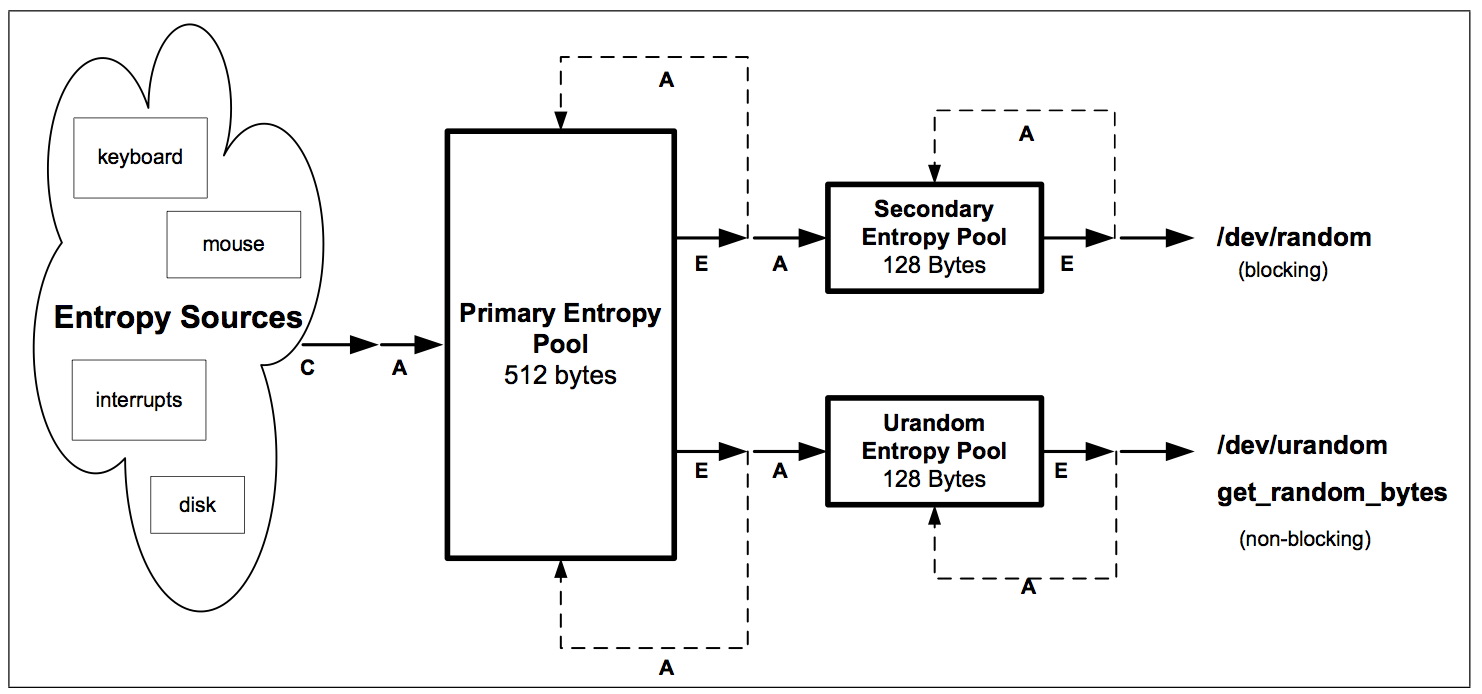
\includegraphics[scale=0.27]{prng.png}
\end{center}
\caption{{\bf General Structure of Linux PRNG}}
\label{figprng}
\end{figure}


The Linux PRNG consists of three entropy pools which act in a same manner. They have two major functions: mix entropy into the pool and extract entropy from the pool. The input pool (also known as the primary pool) gets entropy from three types of entropy sources: disk, interrupt and input. When an event happens in a source, the source feed the timing and the type of the event to the input pool. The two output pools (secondary pools) gets their entropy by extracting entropy from the input pool. The blocking pool blocks upon no entropy in its pool and the input pool while the non-blocking pool does not. An important property of the non-blocking pool is that it does not extract any entropy if the amount of entropy in the input pool is less than 192 (CITE: random.c). When there is no entropy mixed into the non-blocking pool, its output is deterministic and predictable given any of its internal states between the last entropy mix and the time of present. 

The three pools are initialized when the kernel initializes the random character device. On initialization, the pools are not wiped and the time and machine information are mixed in. Under traditional Linux environment, there is an init script which read the saved random seed from the disk and mix it into the nonblocking pool.

%A paragraph of text goes here.  Lots of text.  Plenty of interesting
%text. \\

%More fascinating text. Features\endnote{Remember to use endnotes, not footnotes!} galore, plethora of promises.\\

The rest of the paper is organized as follows. In section 2, we introduce existing work on analyzing Linux PRNG and the low entropy issue, as well as the work aiming at exploiting or defending buffer overflow. Section 3 describes our investigation methodology. Section 4 shows the result of our investigation, revailing several vulnerabilities. In Section 5 we discuss the effect of these vulnerabilities and possible attacks and defenses. Finally, in section 6 we describe the future work.
